%%%%%%%%%%%%%%%%%%%%%%%%%%%%%%%%%%%%%%%%%%%%%%%%%%%%%%%%%%%%%%%%%%%%%%%%%
\section{Maximum-Likelihood Estimation}  %%%%%%%%%%%%%%%%%%%%%%%%%%%%%%%%
\label{cr:app:maxlik}

In this section, we go into the analysis of the ML estimator in depth.
From the definition of choice probabilities in~\eqref{cr:eq:wsinglelik}, it is clear that the likelihood is invariant to a rescaling of the parameters, i.e., $\ell(\bm{\lambda}; \mathcal{D}) = \ell(s \bm{\lambda}; \mathcal{D})$ for any $s > 0$.
We will therefore identify parameters up to rescaling.

%%%%%%%%%%%%%%%%%%%%%%%%%%%%%%%%%%%%%%%%%%%%%%%%%%%%%%%%%%%%%%%%%%%%%%%%%
\subsection{Necessary and Sufficient Conditions}

In order to provide a data-dependent, necessary and sufficient condition that guarantees that the ML estimate is well-defined, we extend the definition of comparison hypergraph presented in Section~\ref{cr:sec:maxlik}.

\begin{definition}[Comparison graph]
Let $G = (V, E)$ be a directed graph and $\{ a_{ij} \mid (i,j) \in E \}$ be non-negative numbers.
The \emph{comparison graph} induced by $\{ a_{ij} \}$ is the directed graph $H = (V, E')$, where $(i,j) \in E'$ if and only if there is a node $k$ such that $i, j \in N^+_k$ and $a_{kj} > 0$.
\end{definition}

The numbers $\{ a_{ij}\}$ can be loosely interpreted as transition counts (although they do not need to be integer).
Intuitively, there is an edge $(i, j)$ in the comparison graph whenever there is at least one instance in which $i$ and $j$ were among the alternatives and $j$ was selected.
If $a_{ij} > 0$ for all edges, then the comparison graph is equivalent to its hypergraph counterpart, in that every hyperedge induces a clique in the comparison graph.
As shown by the next theorem, the notion of (data-dependent) comparison graph leads to a precise characterization of whether the ML estimate is well-defined or not.

\begin{theorem}
\label{cr:thm:mlboth}
Let $G = (V, E)$ be a directed graph and $\{ (c^-_i, c^+_i) \}$ be the aggregate number of transitions arriving in and originating from $i$, respectively.
Let $\{ a_{ij} \}$ be any set of non-negative real numbers that satisfy
\begin{align*}
\sum_{j \in N^-_i} a_{ji} = c^-_i, \quad
\sum_{j \in N^+_i} a_{ij} = c^+_i.
\end{align*}
Then, the maximizer of the log-likelihood~\eqref{cr:eq:wloglik} exists and is unique (up to rescaling) if and only if the comparison graph induced by $\{ a_{ij} \}$ is strongly connected.
\end{theorem}

The proof borrows from \citet{hunter2004mm}, in particular from the proofs of Lemmas~$1$ and~$2$.

\begin{proof}
The log-likelihood~\eqref{cr:eq:wloglik} is not concave in $\bm{\lambda}$, but it can be made concave using the reparametrization $\lambda_i = e^{\theta_i}$.
We can rewrite the reparametrized log-likelihood using $\{ a_{ij} \}$ as
\begin{align*}
    \ell(\bm{\theta})
        = \sum_{i = 1}^n \sum_{j \in N^+_i} a_{ij} \bigg[ \theta_j - \log \sum_{k \in N^+_i} w_{ik} e^{\theta_k} \bigg],
\end{align*}
and, without loss of generality, we can assume that $\sum_i \theta_i = 0$ and $\min_{ij} w_{ij} = 1$.

First, we shall prove that the super-level set $\{ \bm{\theta} \mid \ell(\bm{\theta}) \ge c \}$ is bounded and compact for any $c$, if and only if the comparison graph is strongly connected.
The compactness of all super-level sets ensures that there is at least one maximizer.
Pick any unit vector $\bm{u}$ such that $\sum_i u_i = 0$, and let $\bm{\theta} = s \bm{u}$
When $s \to \infty$, then $e^{\theta_i} > 0$ and $e^{\theta_j} \to 0 $ for some $i$ and $j$.
As the comparison graph is strongly connected, there is a path from $i$ to $j$, and along this path there must be two consecutive nodes $i', j'$ such that $e^{\theta_{i'}} > 0$ and $e^{\theta_{j'}} \to 0$.
The existence of the edge $(i',j')$ in the comparison graph means that there is a $k$ such that $i', j' \in N^+_k$ and $a_{kj'} > 0$.
Therefore, the log-likelihood can be bounded as
\begin{align*}
\ell(\bm{\theta})
    \le a_{kj'} \bigg[ \theta_{j'} - \log \sum_{q \in N^+_k} w_{kq} e^{\theta_q} \bigg]
    \le a_{kj'} \left[ \theta_{j'} - \log (e^{\theta_{j'}} + e^{\theta_{i'}}) \right],
\end{align*}
and $\lim_{s \to \infty} \ell(\bm{\theta}) = -\infty$.
Conversely, suppose that the comparison graph is not strongly connected and partition the vertices into two non-empty subsets $S$ and $T$ such that there is no edge from $S$ to $T$.
Let $c > 0$ be any positive constant, and take $\tilde{\theta}_i = \theta_i + c$ if $i \in S$ and $\tilde{\theta}_i = \theta_i$ if $i \in T$ (renormalize such that $\sum_i \tilde{\theta}_i = 0$).
Clearly, $\ell(\tilde{\bm{\theta}}) \ge \ell(\bm{\theta})$, and by repeating this procedure $\lVert \bm{\theta} \rVert$ may be driven to infinity without decreasing the likelihood.

Second, we shall prove that if the comparison graph is strongly connected, the log-likelihood is strictly concave (in $\bm{\theta}$).
In particular, for any $p \in (0,1)$,
\begin{align}
\label{cr:eq:strictconcav}
\ell \left[ p \bm{\theta} + (1-p) \bm{\eta} \right] \ge p \ell(\bm{\theta}) + (1-p) \ell(\bm{\eta}),
\end{align}
with equality if and only if $\bm{\theta} \equiv \bm{\eta}$ up to a constant shift.
Strict concavity ensures that there is at most one maximizer of log-likelihood.
We start with Hölder's inequality, which implies that, for positive $\{ x_k \}$ and $\{ y_k \}$, and $p \in (0,1)$,
\begin{align*}
\log \sum_k x_k^p y_k^{1-p} \le p \log \sum_k x_k + (1-p) \log \sum_k y_k.
\end{align*}
with equality if and only $x_k = c y_k$ for some $c > 0$.
Letting $x_k = w_{ik} e^{\theta_k}$ and $y_k = w_{ik} e^{\eta_k}$, we find that for all $i$
\begin{align}
\label{cr:eq:holderapp}
\begin{aligned}
\log \sum_{k \in N^+_i} w_{ik} e^{p \theta_k + (1-p) \eta_k}
    \le p \log\!\sum_{k \in N^+_i}\!w_{ik} e^{\theta_k} + (1-p) \log\!\sum_{k \in N^+_i}\!w_{ik} e^{\eta_k},
\end{aligned}
\end{align}
with equality if and only if there exists $c \in \mathbf{R}$ such that $\theta_k = \eta_k + c$ for all $k \in N^+_{i}$.
Multiplying by $a_{ij}$ and summing over $i$ and $j$ on both sides of~\eqref{cr:eq:holderapp} shows that the log-likelihood is concave in $\bm{\theta}$.
Now, consider any partition of the vertices into two non-empty subsets $S$ and $T$.
Because the comparison graph is strongly connected, there is always $k \in V$, $i \in S$ and $j \in T$ such that $i, j \in N^+_k$ and $a_{ki} > 0$.
Therefore, the left and right side of~\eqref{cr:eq:strictconcav} are equal if and only if $\bm{\theta} \equiv \bm{\eta}$ up to a constant shift.

Bounded super-level sets and strict concavity form necessary and sufficient conditions for the existence and uniqueness of the maximizer.
\end{proof}

We now give a proof for Theorem~\ref{cr:thm:mlnecessary}, presented in the main body of text.

\begin{proof}[Proof of Theorem~\ref{cr:thm:mlnecessary}]
If the comparison hypergraph is disconnected, then for any data $\mathcal{D}$, the (data-induced) comparison graph is disconnected too.
Furthermore, the connected components of the comparison graph are subsets of those of the hypergraph.
Partition the vertices into two non-empty subsets $S$ and $T$ such that there is no hyperedge between $S$ to $T$ in the comparison hypergraph.
Let $A = \{ i \mid N^+_i \subset S \}$ and $B = \{ i \mid N^+_i \subset T \}$.
By construction of the comparison hypergraph, $A \cap B = \varnothing$ and $A \cup B = V$.
The log-likelihood can be therefore be rewritten as
\begin{align*}
\ell(\bm{\theta}) =
    \sum_{i \in A} \sum_{j \in N^+_i} a_{ij} \bigg[ \log \lambda_j - \log \sum_{k \in N^+_i} w_{ik} \lambda_k \bigg]
    + \sum_{i \in B} \sum_{j \in N^+_i} a_{ij} \bigg[ \log \lambda_j - \log \sum_{k \in N^+_i} w_{ik} \lambda_k \bigg].
\end{align*}
The sum over $A$ involves only parameters related to nodes in $S$, while the sum over $B$ involves only parameters related to nodes in $T$.
Because the likelihood is invariant to a rescaling of the parameters, it is easy to see that we can arbitrarily rescale the parameters of the vertices in either $S$ or $T$ without affecting the likelihood.
\end{proof}

\begin{figure*}[t]
  \begin{subfigure}{.33\textwidth}
    \centering
    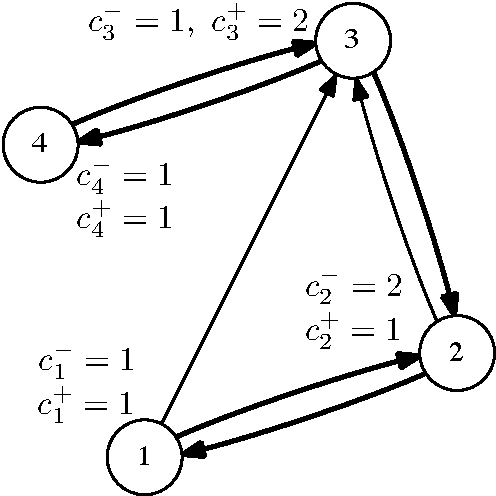
\includegraphics[width=.85\linewidth]{cr-ml-undefined}
    \caption{network structure}
  \end{subfigure}%
  \begin{subfigure}{.33\textwidth}
    \centering
    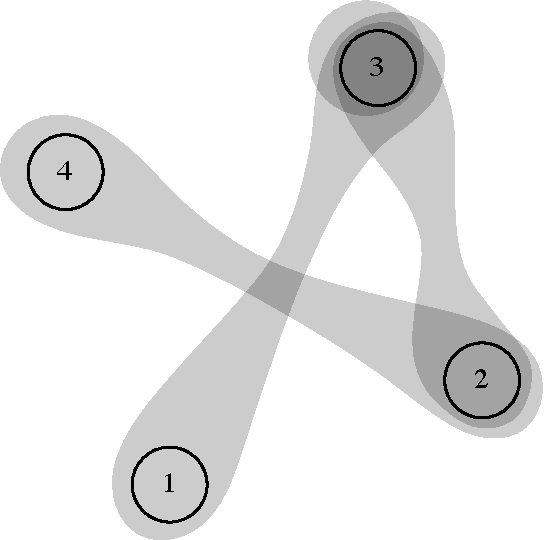
\includegraphics[width=.85\linewidth]{cr-ml-undefined-hyp}
    \caption{comparison hypergraph}
  \end{subfigure}
  \begin{subfigure}{.33\textwidth}
    \centering
    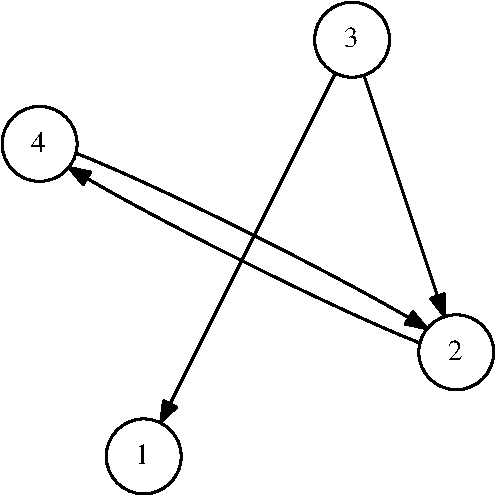
\includegraphics[width=.85\linewidth]{cr-ml-undefined-comp}
    \caption{comparison graph}
  \end{subfigure}
  \caption{An innocent-looking example where the ML estimate does not exist.
  The network structure, aggregate traffic data and compatible transitions are shown on the left.
  While the comparison hypergraph is connected, the (data-dependent) comparison graph is not strongly connected.}
  \label{cr:fig:badexample}
\end{figure*}

\paragraph{Verifying the condition of Theorem~\ref{cr:thm:mlboth}.}
In order to verify the necessary and sufficient condition given $\{ (c^-_i, c^+_i) \}$, one has to find a non-negative solution $\{ a_{ij} \}$ to the system of equations
\begin{align*}
\sum_{j \in N^-_i} a_{ji} &= c^-_i, \\
\sum_{j \in N^+_i} a_{ij} &= c^+_i.
\end{align*}
\citet{dines1926positive} presents a remarkably simple algorithm to find such a non-negative solution.
Alternatively, \citet{kumar2015inverting} suggest recasting the problem as one of maximum flow in a network.
However, the computational cost of running \citeauthor{dines1926positive}' or max-flow algorithms is significantly greater than that of running ChoiceRank.

\subsection{Example}

To conclude our discussion, we provide an innocuous-looking example that highlights the difficulty of dealing with the ML estimate.
Consider the network structure and traffic data depicted in Figure~\ref{cr:fig:badexample}.
The network is strongly connected, and its comparison hypergraph is connected as well; as such, the network satisfies the necessary condition stated in Theorem~\ref{cr:thm:mlnecessary} in the main text.
Nevertheless, the condition is not sufficient for the ML-estimate to be well-defined.
In this example, the (data-dependent) comparison graph is \emph{not} strongly connected, and it is easy to see that the likelihood can always be increased by increasing $\lambda_1$, $\lambda_2$ and $\lambda_4$.
Hence, the ML estimate does not exist.

In this simple example, we indicate the edge transitions that generated the observed marginal traffic in bold.
Given this information, the comparison graph is easy to find, and the necessary and sufficient conditions of Theorem~\ref{cr:thm:mlboth} are easy to check.
But in general, finding a set of transitions that is compatible with given marginal per-node traffic data is computationally expensive (see discussion above).
